\def\year{2022}\relax
%File: formatting-instructions-latex-2022.tex
%release 2022.1
\documentclass[letterpaper]{article} % DO NOT CHANGE THIS
\usepackage{aaai22}  % DO NOT CHANGE THIS
\usepackage{times}  % DO NOT CHANGE THIS
\usepackage{helvet}  % DO NOT CHANGE THIS
\usepackage{courier}  % DO NOT CHANGE THIS
\usepackage[hyphens]{url}  % DO NOT CHANGE THIS
\usepackage{graphicx} % DO NOT CHANGE THIS
\urlstyle{rm} % DO NOT CHANGE THIS
\def\UrlFont{\rm}  % DO NOT CHANGE THIS
\usepackage{natbib}  % DO NOT CHANGE THIS AND DO NOT ADD ANY OPTIONS TO IT
\usepackage{caption} % DO NOT CHANGE THIS AND DO NOT ADD ANY OPTIONS TO IT
\DeclareCaptionStyle{ruled}{labelfont=normalfont,labelsep=colon,strut=off} % DO NOT CHANGE THIS
\frenchspacing  % DO NOT CHANGE THIS
\setlength{\pdfpagewidth}{8.5in}  % DO NOT CHANGE THIS
\setlength{\pdfpageheight}{11in}  % DO NOT CHANGE THIS
%
% These are recommended to typeset algorithms but not required. See the subsubsection on algorithms. Remove them if you don't have algorithms in your paper.
\usepackage{algorithm}
\usepackage{algorithmic}

%
% These are are recommended to typeset listings but not required. See the subsubsection on listing. Remove this block if you don't have listings in your paper.
\usepackage{newfloat}
\usepackage{listings}
\lstset{%
	basicstyle={\footnotesize\ttfamily},% footnotesize acceptable for monospace
	numbers=left,numberstyle=\footnotesize,xleftmargin=2em,% show line numbers, remove this entire line if you don't want the numbers.
	aboveskip=0pt,belowskip=0pt,%
	showstringspaces=false,tabsize=2,breaklines=true}
\floatstyle{ruled}
\newfloat{listing}{tb}{lst}{}
\floatname{listing}{Listing}
%
%\nocopyright
%
% PDF Info Is REQUIRED.
% For /Title, write your title in Mixed Case.
% Don't use accents or commands. Retain the parentheses.
% For /Author, add all authors within the parentheses,
% separated by commas. No accents, special characters
% or commands are allowed.
% Keep the /TemplateVersion tag as is
\pdfinfo{
/Title Multiagent Reinforcement Learning for Traffic Signal Control
/Author Kevyn Kelso
/TemplateVersion (2022.1)
}

% DISALLOWED PACKAGES
% \usepackage{authblk} -- This package is specifically forbidden
% \usepackage{balance} -- This package is specifically forbidden
% \usepackage{color (if used in text)
% \usepackage{CJK} -- This package is specifically forbidden
% \usepackage{float} -- This package is specifically forbidden
% \usepackage{flushend} -- This package is specifically forbidden
% \usepackage{fontenc} -- This package is specifically forbidden
% \usepackage{fullpage} -- This package is specifically forbidden
% \usepackage{geometry} -- This package is specifically forbidden
% \usepackage{grffile} -- This package is specifically forbidden
% \usepackage{hyperref} -- This package is specifically forbidden
% \usepackage{navigator} -- This package is specifically forbidden
% (or any other package that embeds links such as navigator or hyperref)
% \indentfirst} -- This package is specifically forbidden
% \layout} -- This package is specifically forbidden
% \multicol} -- This package is specifically forbidden
% \nameref} -- This package is specifically forbidden
% \usepackage{savetrees} -- This package is specifically forbidden
% \usepackage{setspace} -- This package is specifically forbidden
% \usepackage{stfloats} -- This package is specifically forbidden
% \usepackage{tabu} -- This package is specifically forbidden
% \usepackage{titlesec} -- This package is specifically forbidden
% \usepackage{tocbibind} -- This package is specifically forbidden
% \usepackage{ulem} -- This package is specifically forbidden
% \usepackage{wrapfig} -- This package is specifically forbidden
% DISALLOWED COMMANDS
% \nocopyright -- Your paper will not be published if you use this command
% \addtolength -- This command may not be used
% \balance -- This command may not be used
% \baselinestretch -- Your paper will not be published if you use this command
% \clearpage -- No page breaks of any kind may be used for the final version of your paper
% \columnsep -- This command may not be used
% \newpage -- No page breaks of any kind may be used for the final version of your paper
% \pagebreak -- No page breaks of any kind may be used for the final version of your paperr
% \pagestyle -- This command may not be used
% \tiny -- This is not an acceptable font size.
% \vspace{- -- No negative value may be used in proximity of a caption, figure, table, section, subsection, subsubsection, or reference
% \vskip{- -- No negative value may be used to alter spacing above or below a caption, figure, table, section, subsection, subsubsection, or reference

\setcounter{secnumdepth}{0} %May be changed to 1 or 2 if section numbers are desired.

% The file aaai22.sty is the style file for AAAI Press
% proceedings, working notes, and technical reports.
%

% Title

% Your title must be in mixed case, not sentence case.
% That means all verbs (including short verbs like be, is, using,and go),
% nouns, adverbs, adjectives should be capitalized, including both words in hyphenated terms, while
% articles, conjunctions, and prepositions are lower case unless they
% directly follow a colon or long dash
\title{Multiagent Reinforcement Learning for Traffic Signal Control}
\author{
    %Authors
    % All authors must be in the same font size and format.
    Kevyn Kelso
}
\affiliations{
    %Afiliations
    University of Colorado-Colorado Springs\\
    % If you have multiple authors and multiple affiliations
    % use superscripts in text and roman font to identify them.
    % For example,

    % Sunil Issar, \textsuperscript{\rm 2}
    % J. Scott Penberthy, \textsuperscript{\rm 3}
    % George Ferguson,\textsuperscript{\rm 4}
    % Hans Guesgen, \textsuperscript{\rm 5}.
    % Note that the comma should be placed BEFORE the superscript for optimum readability
    1420 Austin Bluffs Pkwy\\
    Colorado Springs, CO 80919\\

    % email address must be in roman text type, not monospace or sans serif
    kkelso@uccs.edu
%
% See more examples next
}

\begin{document}

\maketitle


% - problem definition
% - problem complexity
% - why it's important
%- what benefits to using RL to solve it
% - introduce SUMO environment and benchmark systems

% To talk about:
% ault2021reinforcement
% - https://people.engr.tamu.edu/guni/Papers/NeurIPS-signals.pdf
% - 12–55% of commute travel time is due to delays induced by signalized intersections (stopped or approach delay)
% - an efficient traffic signal depends on an accurate estimation of the time it takes to travel between the two.
% - introduce Simulation of Urban Mobility traffic simulator (SUMO) and how its evaluated and calibrated by the general transportation community
% - REinforced Signal COntrol or RESCO is a testbed and benchmark environment for comparison between RL-based signal control algorithms
% - tate of the intersection is usually defined by the set of incoming vehicles (incoming lane, speed, waiting time, queue position) and the current signal (right-of-passage) assignmen
% - Such an approach showed a potential reduction of up to 73% in vehicle delays when compared to fixed-time actuation
% - do research on different reward functions (total delays imposed by the intersection, waiting time at the intersection, traffic pressure)
% - Baseline controllers: Fixed time, max pressure, greedy
% - RL algorithms: IDQN (best), IPPO, MPLight, Extended MPLight
% - decentralized control algorithms may be better than centralized
% - performance was overal worse with more environment information except in the dense city example

% - DBLP:journals/corr/abs-2004-04778
% - file:///home/vyn/Downloads/peerj-cs-575.pdf
% - Partial observability may cause distinct states (in which distinct actions are optimal) to be seen as the same by the traffic signal agent
% - partially obeservable variables change the context of the environment and can include: different traffic patterns in different parts of the day, accidents, road maintenence, weather, actions taken by other agents, and other hazards. This is known as non-stationarity
% - Model-free methods, on the other hand, do not require that the agent have access to information about how the environment works. Instead, they learn an action-value function based only on samples obtained by interacting with the environment. we will be using a model free agent
% - Equations on state formulation. State is commonly limited by cost and availability of sensors in the real world (can model how much improvement can be made if new sensors are installed to make better informed decisions on what infrastructure to purchase?)
% - Typically, simulation time steps correspond to 5-10 seconds of actual traffic simulation because signals do not change on a per second basis.
% - change and keep actions, change comes with a yellow phase of 2 seconds.
% - Multiagent allows for different behaviors between agents and avoids the curse of dimensionality that a centralized training scheme would introduce. However, agents learning and adjusting policies results in changes in the environment dynamics which causes non-stationarity. The best policy for an agent changes as the policies for other agents change.
% - context changes such as an accident increasing the queues of an agent can cause an agent to undergo a readaptation phase to correctly update their policies to deal with the context change which results in periods of catastrophic drops in performance.
% - this paper tested introducing different contexts by changing the rate at which cars entered different sides of a 4 x 4 grid traffic scenario
% - In order to obtain a good performance using fixed policies, it would be necessary to define a policy for each context and to know in advance the exact moment when context changes will occur. Moreover, there may be an arbitrarily large number of such contexts, and the agent, in general, has no way of knowing in advance how many exist.
% - exploration and exploitation: exploration allows agents to adapt to context changes
% -  density attributes are fundamental to better characterize the true state of a traffic intersection. they found that only using queue attributes allowed the policy to converge faster due to the smaller state space, but did not perform as well as queue + density in the end.
% - agents might learn actions that apply to both contexts, this is what we want
% - More state observability helps avoid the negative impacts of non-stationarity.
% - Although they used tabular Q learning methods, they believe the non-stationarity also affects DRL algorithms

% - Ghanadbashi2023
% - file:///home/vyn/Downloads/HandlingUncertaintyinSelf-adaptiveSystems_AnOntology-basedReinforcementLearningModel.pdf
% - however, the current mechanisms do not address rare events in an environmen
% - An ontology is a formal specification of a conceptualization of a domain and the relationships between those concepts. [15],
% - Self Adaptive Systems (SAS)
% - . To capture the underlying uncertainty and variability of dynamic environments, the knowledge model can be formulated as a stochastic dynamic decision problem generally modeled via a POMDP and can be solved using an RL framework. 
% - action masking (primarily filtering out invalid or impossible actions) can be used to improve exploration performance
% - based on the distribution of unanticipated events, they can switch between an ontology based policy and an RL based policy
% - they used an augmented reward signal based on the calculated efficiency of each action
% - they suggest state could be augemented by having detectable vehicles in the system so the traffic controller can know information about the vehicle (emergency vehicle, type of vehicle, length, weight, etc...)
% - they create a table of inference rules (ontology rules) to mask observations (masking irrelavant info can improve performance)
% - RL systems do not perform well handling rare events

%- choi1999environment
% - https://proceedings.neurips.cc/paper_files/paper/1999/file/e8d92f99edd25e2cef48eca48320a1a5-Paper.pdf
% - traditional MDPs assume dynamics of the environment don't change. Classically, elevators are non-stationary
% - non-stationary environments don't come with convergence guarantees that traditional MDPs have
% - must be some regularity in the way the environment changes
% - propose to add "modes" or contexts in addition to the state
% - Basically you have an MDP for each mode, and a way to detect which mode you are in
% - Modes can be modeled in a traffic simulator environment by assigning fixed probabilities for cars waiting at each direction of the intersection, then changing those probabilities in discrete steps for example just switching them
% - agents actions do not affect modes in TSC
% - mode changes are infrequent and number of states are substantially larger than modes

% - hafiz2020deep
% - https://arxiv.org/pdf/2008.04109.pdf
% - shared state and rewards, but agent specific action updating in the experience replay pools = simplicity, faster convergence, and better performance than baseline models
% - non-linear Q functions showed to not perform well due to correlations in the sequence of states, small updates to Q significantly changing the policy
% - experience replay in DQN helps get rid of the correlations by randomizing the experience data used for further training of the network
% - inter-agent communication is complex
% - There are many types of DQN, LDQN, HDQN, WDDQN, DPIQN, DRPIQN
% - binary DQN: each agent corresponds to a possible action the system can take 0 = no action, 1 = take action. AKA CS-DQN
% - simple typically yeilds better performance

% - 10.3389/frai.2022.805823
% - centralized control is intractable for TSC, centralized training, decentralized execution
% - agents typically share the same reward function in cooperative environments, every agent deduces its own contributions based on the team reward
% - having each agent learning independently where each agent treats the others as part of the environment is a bad idea because from each agents perspective, the dynamics appear non-stationary due to other agents learning
% - parameter sharing can be utilized for all independent agents. experience from all agents are trained simultaneously using a single network
% - PPO is highly sensitive to environment and hyperparameters

% - Almeida2022MultiagentRL
% - This relates closely to multiagent systems and to multiagent reinforcement learning, as many problems in traffic management and control are inherently distributed.
% - State space is large and continuous, making it more difficult to properly discretize states, cuasing algorithms to converge more slowly.
% - air pollution, decrease in speed, delays, opportunity costs
% - function approximation comes with some drawbacks including They make the learning harder to comprehend, and generally require that the agents gather a large amount of data to be able to successfully generalize and apply their collected experiences.
% - One of these strategies is 𝜀-greedy, where an action is randomly chosen (exploration) with a probability 𝜀, or, with probability 1-𝜀, the best known action is chosen, i.e., the one with the highest Q-value so far (exploitation).
% - in many real-world problems, where the control is decentralized, there is no way to avoid a multiagent RL formulation
% - uses a 4x4 grid network of traffic lights
% - experimented with link length between traffic lights
% - raffic signals in our scenario have a minimum and maximum time they must remain green. They are referred to as minGreenTime and maxGreenTime, respectively
% - has great descriptions of state and action spaces
% - they did the same context experiment as the previous paper

% - Reza2023
% - SARSA lambda, sequences of decisions significantly impact the outcome
% - most traffic lights only have inductive sensors reducing performacne for accuracy and efficiency
% - the multi-agent RL techniques are the current state-of-the-art in managing vehicles within road networks
% - Temporal distance (TD), which may be defined as the difference in values at different times, allows an agent to calculate values in a non-deterministic environment
% - also use same reward function as Almeida2022MultiagentRL
% - the signals follow the cycle even if no vehicles are present currently deployed
% - they used a Guassian function to more effectively decay the eligibility traces

% - DBLP:journals/corr/MnihKSGAWR13
% - Deep neural network trained with an experience replay mechanism [13] which randomly samples previous transitions, and thereby smooths the training distribution over many past behaviors
% - n practice, this basic approach is totally impractical, because the action-value function is estimated separately for each sequence, without any generali- sation. Instead, it is common to use a function approximator to estimate the action-value function, Q(s, a; θ) ≈ Q∗(s, a).
% - model-free: it solves the reinforcement learning task directly using sam-ples from the emulator E
% - off-policy: it learns about the greedy strategy a = maxa Q(s, a; θ), while following a behaviour distribution that ensures adequate exploration of the state spac
% - it was shown that combining model-free reinforcement learning algorithms such as Q- learning with non-linear function approximators [25], or indeed with off-policy learning [1] could cause the Q-network to diverge
% - Since the scale of scores varies greatly from game to game, we fixed all positive rewards to be 1 and all negative rewards to be −1

% - Mnih2015
% - Reinforcement learning is known to be unstable or even to diverge when a nonlinear function approximator such as a neural network is used to represent the action-value (also known as Q) function - 
% - perhaps using a neural network representing only the valid actions in the output would produce better performance. Network could be selected based on valid actions available (binary DQN?)
% - his manner limits the scale of the error derivatives and makes it easier to use the same learning rate across multiple games. 
% - he fact that there is similar structure in the two-dimensional embeddings corresponding to the DQN representation of states experienced during human play (orange points) and DQN play (blue points) suggests that the representations learned by DQN do indeed generalize to data generated from policies other than its own.
% - plotting the value (V) over time, can see spikes in expected value
% - with replay yields an order of magnitute performance increase

\begin{abstract}
Transportation is a complex problem facing developed societies.
It is riddled with logistical challenges extending beyond pollution and traffic congestion.
The idea of applying reinforcement learning to transportation problems is not new but has great potential for improvement and research in the field.
Contrary to current approaches, reinforcement learning can make decisions in stochastic and uncertain environments characteristic of traffic problems.
Many common reinforcement learning approaches have been applied, showing promise over other approaches, and will be compared below.
This project aims to reproduce existing methods and attempt to improve performance concerning the traffic throughput metrics described below.
An integration of various ideas from the literature, combined to study what can be learned from reinforcement learning experimentation with regards to traffic control is the primary purpose.
\end{abstract}

\section{Introduction}
Traffic Signal Control (TSC), a classic control problem affecting all drivers, holds exciting potential for reinforcement learning to address obvious societal problems including air pollution, decreases in speed, delays, and opportunity costs \cite{Almeida2022MultiagentRL}.
Based on travel research conducted in urban areas, 12-55\% of total commute time is caused by signalized intersections (traffic lights) \cite{ault2021reinforcement}.
Moreover, modern reinforcement learning (RL) approaches suggest a potential 73\% reduction in that time compared to traditional approaches currently deployed \cite{ault2021reinforcement}.
The field of traffic signal control contains many ideas to increase traffic efficiency in both the fixed algorithm and RL space.
However, many advanced solutions come with expensive caveats. For instance, installing advanced sensors, reworking road paths, or replacing traffic lights with roundabouts \cite{DBLP:journals/corr/abs-2004-04778}.
This project aims to study reinforcement learning approaches to TSC that can be deployed to existing metropolitan areas with minimal cost and infrastructure changes.
In this paper, we will discuss the TSC problem in terms of the Markov Decision Process (MDP) paradigm; and how it is formally described.
Existing methods will then be explored including what is deployed traditionally in most urban environments, and what RL methods could also be used.
Then, our unique solution will be proposed based on information collected comparing a wide variety of methods used previously on the TSC problem \cite{hafiz2020deep} \cite{ault2021reinforcement} \cite{Ghanadbashi2023}.
Finally, a discussion of evaluation metrics, expected challenges, and the timeline of the project will be discussed.

\section{Problem Formulation}
Multiagent approaches to TSC are Partially Observable Markov Decision Processes (POMDPs) with non-stationary dynamics, placing them in one of the most difficult classes of problems for RL to solve \cite{Almeida2022MultiagentRL} \cite{DBLP:journals/corr/abs-2004-04778} \cite{choi1999environment}.
Non-stationary problems do not come with convergence guarantees of traditional MDPs and the partial observability can cause the agent to miss nuance in the state necessary for optimal policies \cite{choi1999environment} \cite{10.3389/frai.2022.805823}.
State aliasing is common in POMDPs where the agent finds two states that are different to be the same, resulting in inappropriate actions.
Additionally, centralized agent approaches suffer from Bellman's curse of dimensionality, require unfeasible infrastructure modifications, and have shown suboptimal performance in simulation \cite{DBLP:journals/corr/abs-2004-04778} \cite{ault2021reinforcement}.

\subsection{State space}
The state space for traffic signal control is a vector of various traffic-related parameters described below.
In the TSC problem, the state space is typically modeled as~\ref{eq:state_space} where each time step \(t\) corresponds to five seconds of actual traffic dynamics, \(\rho_1\) and \(\rho_2\) are binary variables \(\rho_1, \rho_2 \in {0, 1}\) indicating the state of the intersection lights, \(g\) indicates if the light has been green for the minimum specified time, \(L\) is the list of all lanes with density \(\Delta_l\) which is the number of vehicles in each lane divided by the capacity of that lane.
\(q_l\) is the number of queued vehicles in each lane \(l \in L\) \cite{Almeida2022MultiagentRL}.

\begin{equation}
s_t = [\rho_1, \rho_2, g, \Delta_1, \ldots, \Delta_L, q_1, \ldots, q_L]
\label{eq:state_space}
\end{equation}

In reality, few intersections contain the sensors needed to make up the state space described in~\ref{eq:state_space}, so it will be interesting to explore how state space restriction affects agent performance.

\subsection{Action space}
The action space is best described in figure \ref{fig:action_space} where the green paths indicate where traffic can flow and the red paths are not allowed.
The agent can change the intersection into one of four modes \(a_t \in {a_1, a_2, a_3, a_4}\).
There are two direct flow modes and two turning modes.
In the direct flow modes North to South and East to West, the vehicles are also permitted to take right turns.
To change the intersection into a different mode, a mandatory yellow phase $\phi$ precedes the mode change.
In most simulation scenarios, $\phi$ = 2 seconds.

\begin{figure}[htbp]
  \centering
  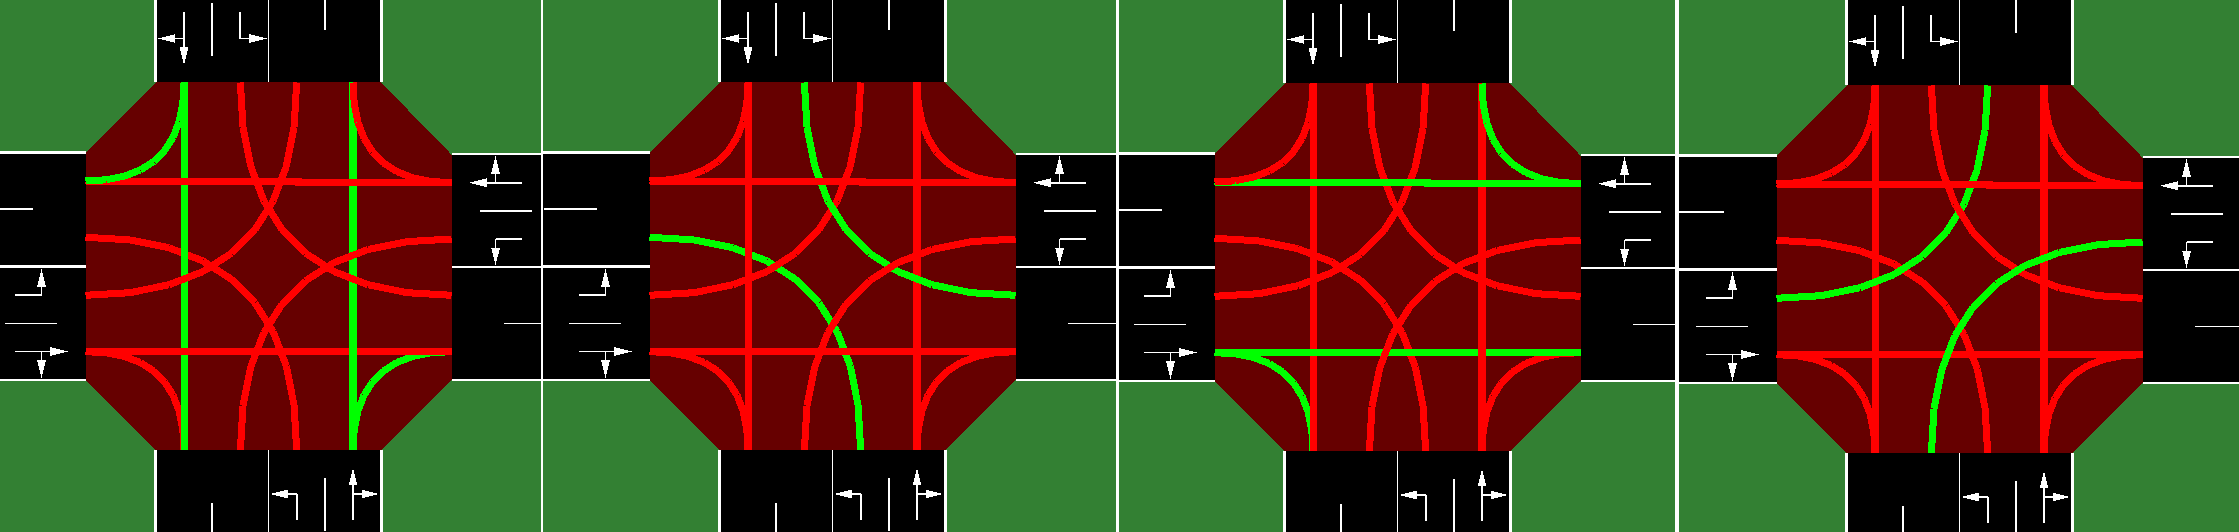
\includegraphics[width=0.8\linewidth]{actions.png}
  \caption{Traffic light modes}
  \label{fig:action_space}
\end{figure}

\subsection{Reward function}
In most papers, the cumulative delay reward function \ref{eq:cumulative_delay} is used where \(D_t\) is the sum of all vehicles wait time \ref{eq:wait_time_sum}.
Other papers extend this idea to the sum of all vehicle wait times in the system to encourage cooperation between agents \cite{10.3389/frai.2022.805823}.
Furthermore, other sophisticated reward functions such as traffic pressure, augmented rewards based on intersection efficiency, and rewards based on ontology adherence have been explored \cite{ault2021reinforcement} \cite{Ghanadbashi2023}.
In this project, the cumulative delay reward function \ref{eq:cumulative_delay} will be used.
However, the cumulative delay will be the sum of all vehicles in the system instead of at the intersection level, where \(V_t\) is the set of all vehicles present in the simulation.
The idea behind this is to encourage the agents to work together rather than develop adversarial relationships.

\begin{equation}
r_t = D_t - D_{t+1}
\label{eq:cumulative_delay}
\end{equation}

\begin{equation}
D_t = \sum_{v \in V_t} d_t^v
\label{eq:wait_time_sum}
\end{equation}

\subsection{Environment Simulator}
The Simulated Urban MObility (SUMO) environment will be used for experimentation because it has been evaluated and calibrated by the general transportation community \cite{ault2021reinforcement} \cite{sumorl} and is widely used in the literature.
Additionally, SUMO was chosen for its compatibility with the OpenAI PettingZoo API which helps create a more standard environment interface for RL systems \cite{terry2021pettingzoo}.
A 4 x 4 grid structure \ref{fig:intersection_grid} of traffic lights will be used as it is also widely used by other papers \cite{Almeida2022MultiagentRL} and is easily understood.
This will necessitate 16 independent agents.
As a future work item, studying how agents trained on a 4 x 4 grid environment transfer to more complex environments such as the cities of Cologne or Ingolstadt will be interesting.

\begin{figure}[htbp]
  \centering
  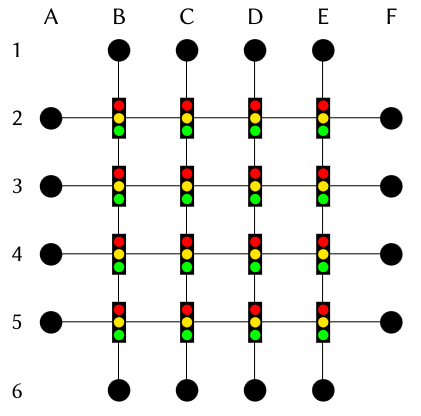
\includegraphics[width=0.6\linewidth]{4x4.png}
  \caption{4 x 4 intersection grid}
  \label{fig:intersection_grid}
\end{figure}

\section{Existing Methods}
\subsection{Traditional Controllers}
The traffic controllers currently used in most areas today fall into three categories of algorithms: fixed time, max pressure, and greedy.
Fixed time controllers will set the traffic signal into one of the four modes for a fixed amount of time, cycling through each mode \cite{ault2021reinforcement}.
Max pressure is the idea of selecting the traffic flow direction based on subtracting the number of cars after the intersection from the number of cars before the intersection \cite{Chen_Wei_Xu_Zheng_Yang_Xiong_Xu_Li_2020}.
The greedy algorithm selects the mode that allows the direction with maximum queue length through.

\subsection{RL Controllers}
Most popular RL methods have been applied to TSC including Independent Deep Q-Learning Networks (IDQN), Independent Proximal Policy Optimization (IPPO), MPLight (variant of DQN) \cite{Chen_Wei_Xu_Zheng_Yang_Xiong_Xu_Li_2020}, Feudal Multiagent Advantage Actor-Critic (FMA2C, MA2C) \cite{DBLP:journals/corr/abs-1903-04527}, State Action Reward State Action Lambda \(SARSA(\lambda)\), TD methods \cite{Reza2023}, Self Adaptive Systems (SAS), and ontology-based RL models \cite{Ghanadbashi2023}.
Based on the results from each of these papers, IDQN appeared to have the most promising performance, and will be discussed further below.


\begin{table}[H]
\centering
\begin{tabular}{lc}
\hline
\textbf{Method} & \textbf{Average Cumulative Delay (seconds)} \\ \hline
IDQN            & 30.74                  \\
IPPO            & 36.15                  \\
MPLight         & 54.58                  \\
MA2C            & 38.07\footnotemark[1]                  \\
FMA2C           & 42.26                  \\
\(SARSA(\lambda)\)           & 18.00\footnotemark[2]                  \\
Ontology        & 17.00\footnotemark[2]                  \\ \hline
\end{tabular}
\caption{Average Delay Across All Scenarios}
\label{tab:avg_delay}
\end{table}
\footnotetext[1]{Data was only collected in one scenario and may not reflect how the model performs in other scenarios.}
\footnotetext[2]{Data was extracted from graphs.}

\section{Proposed Method}
Based on performance data collected in other studies \cite{ault2021reinforcement} \cite{Ghanadbashi2023},
IDQN is the chosen approach to solve the TSC problem.
IDQN is an off-policy, model-free RL method incorporating the idea of collecting experience tuples as the agent plays episodes.
The experience is then used to train a deep neural network and is randomly shuffled to smooth the training data across many past behaviors \cite{DBLP:journals/corr/MnihKSGAWR13}.
The input to the network is the state information, and the output is a Q-value mapped to each action.
In the past, non-linear Q-value function approximators (such as a deep neural network) were unsuccessful due to correlations in the sequence of states, and small updates to Q significantly changing the policy \cite{hafiz2020deep}.
Experience replay and other DQN methods were shown to significantly increase the chances of convergence and improve performance by an order of magnitude \cite{Mnih2015}.
Additionally, simplifying the deep neural network to output only binary values of whether to take the action or not yielded better performance than mapping a Q-value to each action. This is called binary DQN or CS-DQN \cite{hafiz2020deep}.
Based on this information, a binary DQN agent for each traffic signal intersection will be used to solve the 4x4 grid TSC environment.
An off-policy action selection method known as $\epsilon$-greedy will be used, where $\epsilon$ is the probability the agent will select a random action instead of following the learned policy.
Higher values of $\epsilon$ encourage exploration, while lower values encourage exploitation.
The value of $\epsilon$ does not have to be constant throughout the learning process, and choosing an $\epsilon$ value that decays linearly from 1.0 to 0.1 provided good results \cite{Mnih2015}.

\section{Performance Metrics}
% - RESCO, injected uncertainty, average vehicle wait time
% - REinforced Signal COntrol or RESCO is a testbed and benchmark environment for comparison between RL-based signal control algorithms
REinforced Signal COntrol (RESCO) is a testbed and benchmark environment to help judge the performance of RL-based algorithms for TSC. It comes built-in with the SUMO project and will simulate traffic in the same way it was simulated in other benchmark papers \cite{ault2021reinforcement}. This can be used to compare this project with what has already been done.
The metrics that are relevant to this project include: total wait time for each vehicle, average delay per vehicle, average number of stops, average queue length, and average trip time \cite{Reza2023}.
Studying how the agents respond to injected uncertainty such as an emergency vehicle or increased traffic demands is also an important metric for designing a robust system \cite{DBLP:journals/corr/abs-2004-04778}.
% - total waiting time, the average delay per vehicle, the average number of stops \cite{Reza2023}

\section{Expected Challenges}
The non-stationary nature of multiagent RL problems is known to cause divergence problems due to the constantly changing dynamics.
This can be somewhat mitigated by applying a scenario that is consistent across training, but the dynamics will still be changing due to the other agents' learning \cite{DBLP:journals/corr/abs-2004-04778}.
Introducing context switches by changing the scenario, for example, making vehicles flow in waves to simulate rush hour is critical to designing a robust traffic system, but will be out of the scope of the initial research goals.
% - injecting uncertainty \cite{DBLP}

\section{Timeline}

\begin{table}[H]
\centering
\begin{tabular}{ll}
\hline
\textbf{Date} & \textbf{Milestone}             \\ \hline
2/19 & 4x4 grid environment setup and working  \\
2/26 & IDQN agents learning                    \\
3/4  & Perform experiments and generate data   \\
3/18 & Injected uncertainty scenarios          \\
4/1  & Data compilation and writing            \\ \hline
\end{tabular}
\caption{Project Timeline}
\label{tab:project_timeline}
\end{table}

\section{Conclusion}
Overall, it was discussed how traffic signal control (TSC) can be formulated in the Markov Decision Process (MDP) paradigm. The state, action, and reward spaces were defined.
Based on research done applying fixed algorithm and reinforcement learning to TSC, an Independent Deep Q-Learning Network approach was chosen for continued experiments, aiming to reduce the average cumulative delay \(D_t\) to 30.74 seconds or lower.
The performance will be evaluated using the REinforced Signal Control RESCO toolkit, and simulations will be done on the Simulated Urban MObility SUMO environment.
Given the partial and non-stationary nature of the TSC problem, it is expected to face divergence challenges. Overall, the project will be completed following the Project Timeline table \ref{tab:project_timeline}.

% \appendix
% \section{Reference Examples}
% \label{sec:reference_examples}

%- \nobibliography*
\bibliography{proposal}
% - \bibentry{em:86}.

% Use \bibliography{yourbibfile} instead or the References section will not appear in your paper

\end{document}
